\section{Introduction} 
\label{sec:introduction}

{\em 
The history of all hitherto computer science is the history of a struggle
between isolation, portability and performance. (With apologies to Karl Marx.)}

At the dawn of civilization, applications had access to (and had to manage) raw
hardware.  Portability of code and isolation between applications were distant
dreams in the eyes of a handful of visionaries.  Then came the operating system,
which offered a measure of isolation and portability. As the operating systems
became more sophisticated, and applications demanded more portability and
isolation, deep layering became the norm.  Today, when an application sends
network traffic it does so through the vast and deep TCP/IP stack. The deep
layering significantly improves the application portability (the same code can
be reused on many systems and on many types of physical networks), and offers a
certain degree of isolation among applications (via mechanisms like rate control
implemented in the kernel). However, it has been well
documented~\cite{dcqcn,luigipapers} that the modern TCP/IP stack is vastly
inefficient.

The trend continued further as virtualization gained popularity\footnote{The
roadmap also includes detours to technologies such as managed runtimes and
library operating systems, which follow roughly the same storyline}: it offered
even more isolation, and additional portability (you could pack up and move VMs at
will, even live-migrate them). In return, performance -- especially the network
performance dropped further. 

In each case, as the impact of the performance drop was felt, new techniques
were proposed to trade away degrees isolation and portability, for better
performance. For example, to overcome the performance limitations of TCP/IP,
techniques like RDMA~cite{xxx} and DPDK~{xxx} were developed. These offer better
performance, but with less portability (the code can only run on certain
hardware) and less isolation (the application is more exposed to hardware
vagaries, and kernel cannot provide protections like rate limiting and
firewalls). In case of VMs, techniques like SRiOV~\cite{xxx} and
NetVM~\cite{xxx} pierce through the isolation boundary enforced by the
hypervisor to offer better performance. 

The latest step in this trend is called containerization.  By wrapping a process
into a complete filesystem and namespace cell, a container has everything needed
to run the process, including executables, libraries, system tools,
configurations, etc. A container has no external dependencies, which makes it
highly portable. The namespace of the container is isolated from other
containers, eliminating worries about naming and version conflicts.  Such
portability and independence significantly simplifies the life cycle of a
containerized application, from testing to high availability maintenance.

The question is, what is the performance cost of the isolation and portability
offered by the containers? Ideally, containers on a (bare metal) server should
get the same networking performance as processes on the same (bare metal)
server. However, it turns out that this is not the case, as illustrated in
Figure~\ref{fig:motivation}.  We set up two Docker
containers on a server (XXX CPU, YYY GB of memory, 40Gbps Mellanox CX3 NIC, Ubuntu
XXX) with iPerf and benchmarked the network bandwidth and latency between
them. Containers can be networked in two modes~\footnote{We ignore the third
mode, called "bridge", to keep discussion simple.} 
\begin{itemize}
\item {\em Host}, in which one container binds an interface and a port on the
    host and use the host's IP to communicate, like an ordinary process. The
    containers are not truly isolated, since they must share the port space.
\item {\em Overlay}, in which the host runs a software router which connects
    all containers on the host via bridge network. An overlay network crossing
    multiple hosts is constructed by the software routers to achieve a uniform
    IP assignment and traffic routing on the overlay. This makes containers
    fully portable -- they can even have public IPs assigned to them.
\end{itemize}

\begin{figure}[ht]
     \centering 
     %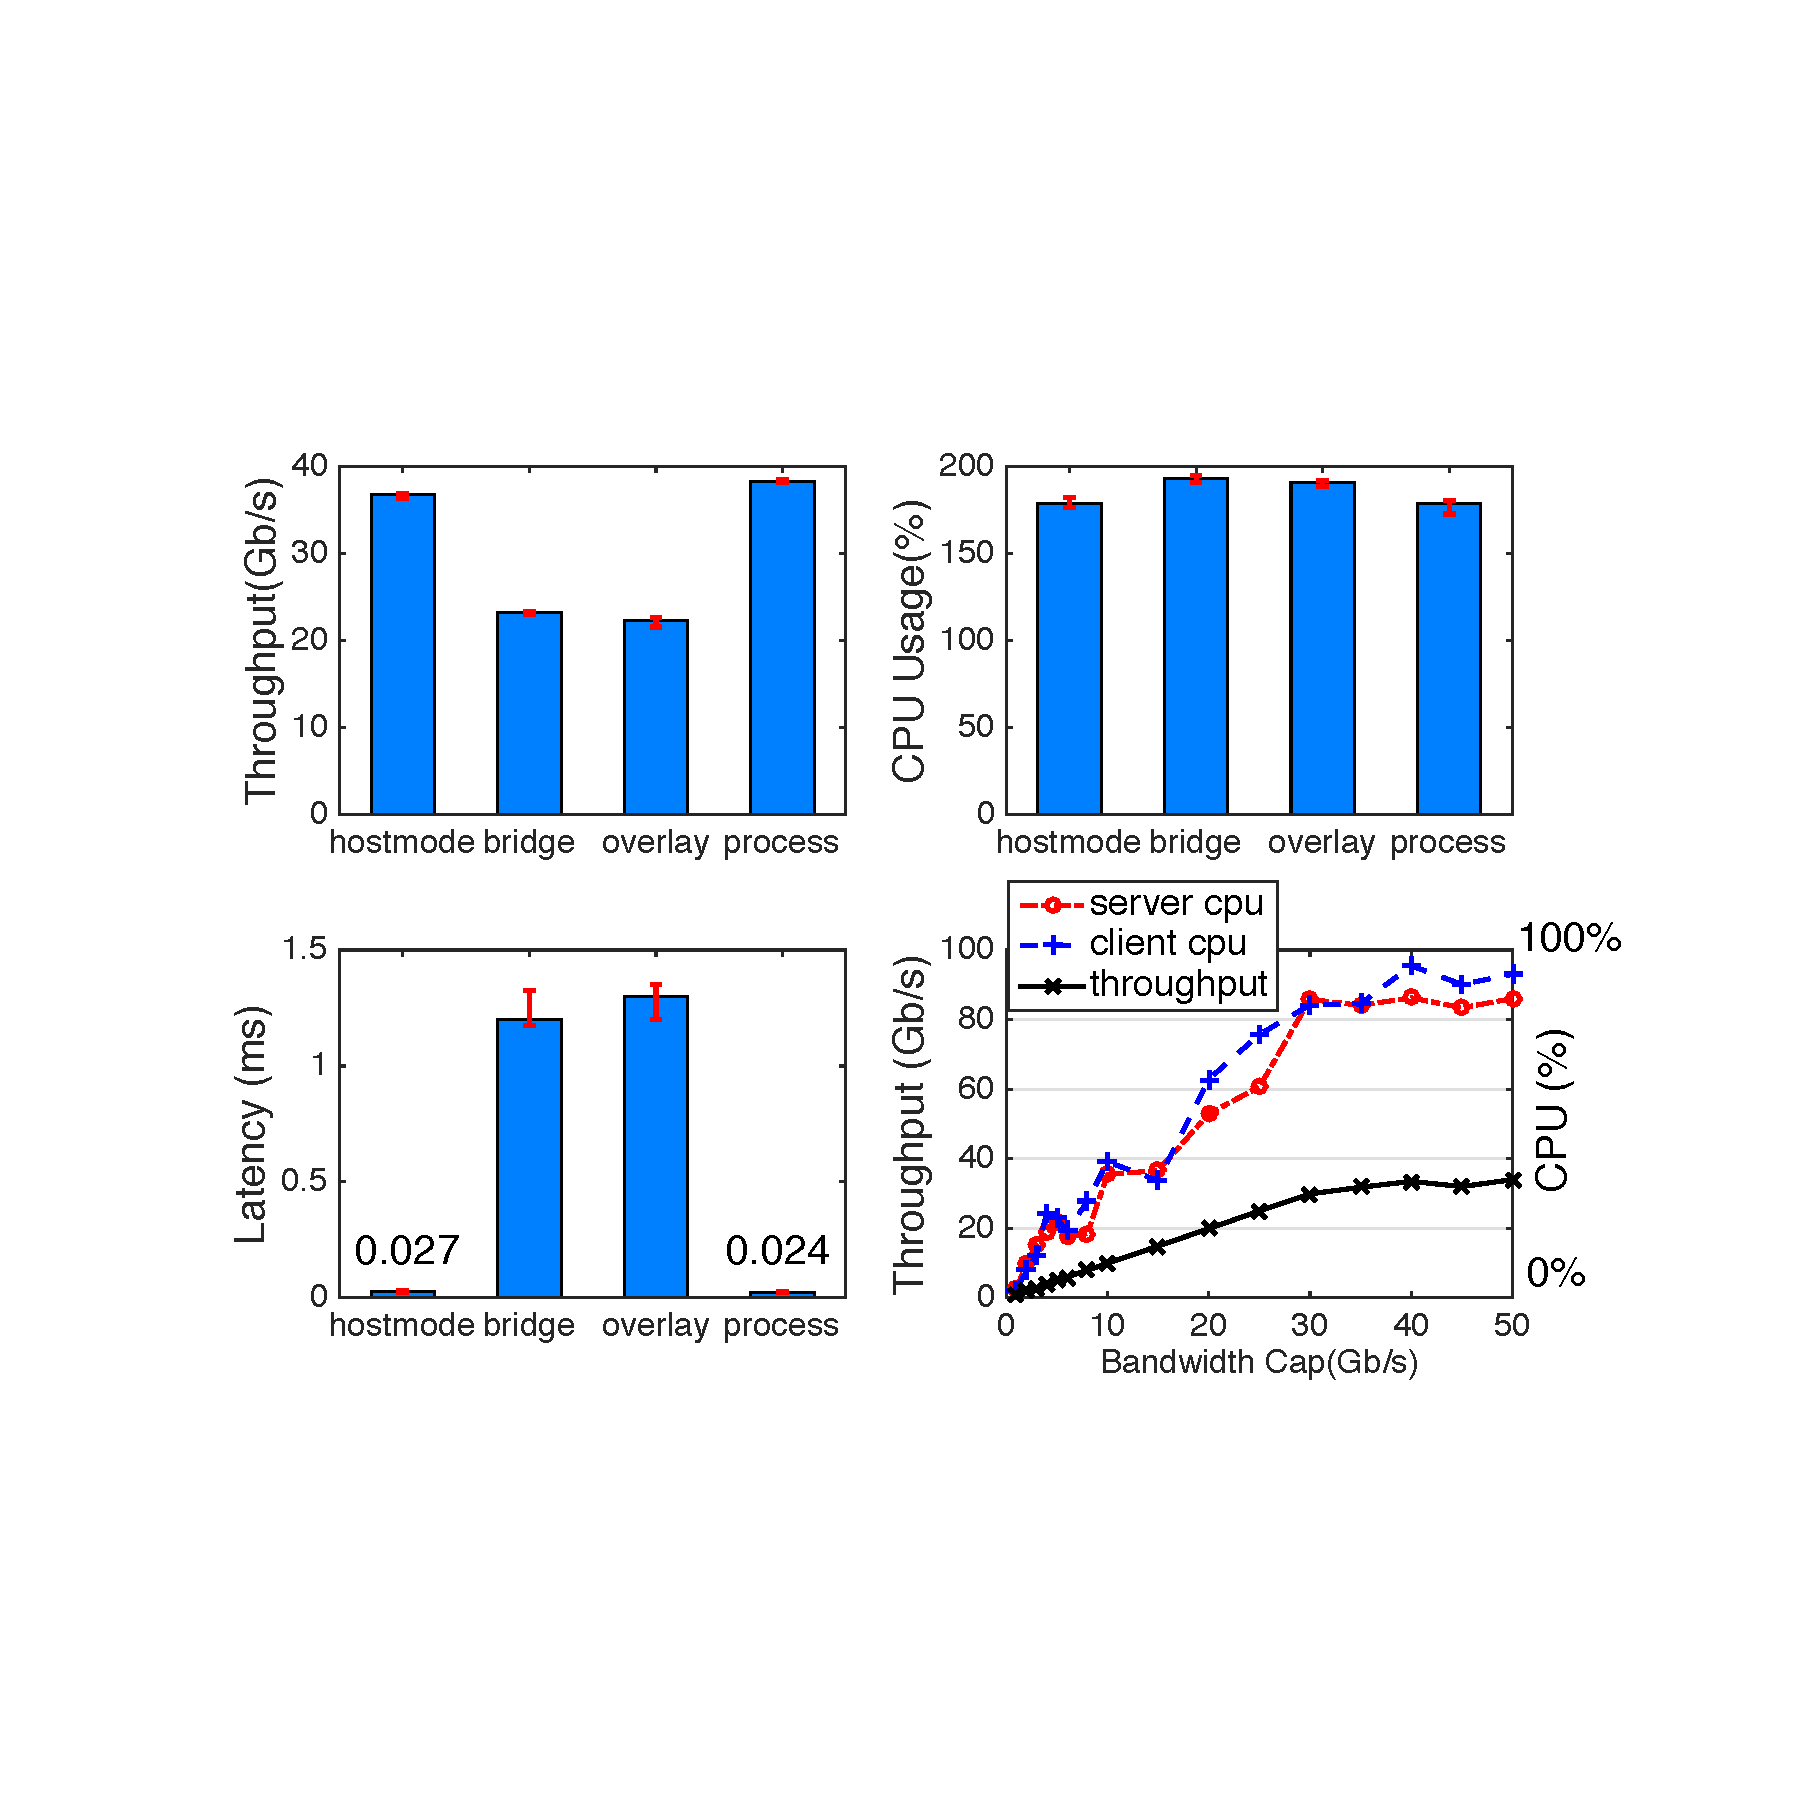
\includegraphics[width=0.5\textwidth]{figures/intro/intro_exist.pdf} 
     \label{fig:three_modes}
     \caption{Performance of two modes of container networking, compared to
     shared memory IPC.} 
\end{figure} 

Figure~\ref{fig:three_modes} shows the median network bandwidth and latency
between two containers with the two networking modes. The error bars show SIQR.
The third bar shows what we can term as the best possible case for two
applications on the same physical server: IPC communication via shared memory.
Needless to say, this mode of communication has the least amount of portability
and isolation.

We make two observations from this figure. First, that the throughput and
latency of both modes of inter-container communication is significantly worse
than best-possible IPC. The reason is obvious: when two containers communication
they have no choice but to ``hairpin'' through the full TCP/IP stack. Second,
the performance of overlay networking is worse than host mode. The reason, again,
is simple: in case of overlay networking, hairpinning happens twice, since the
packets must traverse through the software router as well. This figure thus
clearly illustrates the performance cost of isolation and portability.

As the popularity of container networking grows, this inefficiency must be
addressed. On one hand, the low throughput and high latency directly impacts
the overall performance of large scale distributed systems, such as big data
analytics~\cite{choudhury-paper}, key-value store~\cite{farm}, machine learning
etc.  On the other hand, it forces the applications to reserve substantial CPU
resources to merely perform traffic processing, which significantly raise the
cost of running the applications.

The reader may argue that there is nothing new here: virtualization suffers from
similar inefficiencies and we know how to address them using techniques like
SR-IOV~\cite{sriov} and NetVM~\cite{netvm}.

Unfortunately, these ideas cannot be directly applied to the container world.
SR-IOV typically scales to tens of VMs per server. On the other hand, in typical
deployments, there are hundreds of containers per server. The cost of supporting
so many containers in NIC hardware will be prohibitive. NetVM~\cite{netvm}
cannot be used directly with containers, since it destroys portability -- it
works only when the two VMs are on the same servers. Developers prize containers
especially for their portability: indeed, Docker's main selling point is that a
containerized application that runs on developer's desktop will run in the cloud
without any changes! Another classic solution that trades off portability and
isolation for performance is RDMA. Even that is tricky to use in the container
world. The reason is subtle: containers can indeed use RDMA (i.e. kernel
bypass), but since it requires access to hardware, they have to operate in the
host mode. This means that containers on the same host have to share port space.
This limits their portability, since they need to coordinate with other
containers on the same host to avoid port conflicts.

An ideal solution for container networking is an overlay network with flexible
IP assignment and routing in control-plane and high throughput, low latency and
negligible overhead in data-plane. In this paper, we will discuss the outline of
such a solution. 

Our key idea is to extract information about container location from container
orchestrator (like Mesos), and the fabric controller (if containers are deployed
in public clouds), and then use the appropriate technologies such as RDMA or
shared memory to achieve the best possible performance without any impact
on container portability. Thus, our proposed solution is entirely transparent to
application developers -- they continue to write their applications against
well-known APIs, while our overlay library and coordinator perform the necessary
magic underneath.

In the rest of the paper we discuss the architectural challenges in building
such an overlay network, and outline our design. We have also built a preliminary
version of the system, which we will use to present initial results.
